%-------------------------------------------------------------------------------
\subsubsection{Equivalence des normes}
%-------------------------------------------------------------------------------

Donner des constantes $c_1$ et $c_2$ permettant de comparer les trois normes $\|\cdot\|_1$, $\|\cdot\|_2$ et $\|\cdot\|_\infty$ dans $\Rbb^n$.
\solution{On considère les trois paires de normes.
\begin{description}
  \item[$\|x\|_2$ et $\|x\|_\infty$:] On a vu en cours que
  $$
  \|x\|_\infty \leq \|x\|_2 \leq \sqrt{n} \|x\|_\infty.
%   \qquad \Rightarrow \qquad
%   \frac1{\sqrt{n}} \|x\|_2 \leq \|x\|_\infty \leq \|x\|_2. 
  $$
  \item[$\|x\|_1$ et $\|x\|_\infty$:]  On voit facilement que 
  $$
  \|x\|_\infty \leq \|x\|_1 \leq n \|x\|_\infty.
%   \qquad \Rightarrow \qquad
%   \frac1n \|x\|_1 \leq \|x\|_\infty \leq \|x\|_1.
  $$
  \item[$\|x\|_1$ et $\|x\|_2$:]  On peut déduire une comparaison de $\|x\|_1$ et $\|x\|_2$ en combinant ces résultats
  \begin{align*}
  & \|x\|_1 \leq n \|x\|_\infty \leq n \|x\|_2 \leq n^{3/2} \|x\|_\infty \leq n^{3/2} \|x\|_1 \\
  \Rightarrow \qquad
  & \frac1n \|x\|_1 \leq \|x\|_2 \leq \sqrt{n} \|x\|_1.
%   \Rightarrow \qquad
%   & \frac1{\sqrt{n}} \|x\|_2 \leq \|x\|_1 \leq n \|x\|_2.
  \end{align*}
  On peut cependant affiner les deux constantes :
  \begin{enumerate}
    \item en remarquant que, en définissant les vecteurs $u_i = x_i e_i$ (où les $e_i$ sont les vecteurs de la base canonique), l'inégalité triangulaire implique que
    $$
    \|x\|_2 \leq \sum_i \|u_i\|_2 \leq \sum_i |x_i| = \|x\|_1 ;
    $$
    \item en remarquant que la boule unité de la norme $\|\cdot\|_2$ est incluse dans la boule de rayon $\sqrt{n}$ de la norme $\|\cdot\|_1$, il vient que 
    $$
    \|x\|_1 \leq \sqrt{n} \|x\|_2.
    $$
  \end{enumerate}
\end{description}
  On peut vérifier que les constantes sont optimales en donnant des exemples pour lesquels chacune des égalités est obtenue.
\begin{description}
  \item[$\|x\|_2$ et $\|x\|_\infty$:] Si tous les coordonnées de $x$ sont égales, on a $\|x\|_2 = \sqrt{n} \|x\|_\infty$. \\
  Si tous les coordonnées de $x$ sont nulles, sauf une, on a $\|x\|_2 = \|x\|_\infty$.
  \item[$\|x\|_1$ et $\|x\|_\infty$:] Si tous les coordonnées de $x$ sont égales, on a $\|x\|_1 = n \|x\|_\infty$. \\
  Si tous les coordonnées de $x$ sont nulles, sauf une, on a $\|x\|_1 = \|x\|_\infty$. 
  \item[$\|x\|_1$ et $\|x\|_2$:] Si tous les coordonnées de $x$ sont nulles sauf une, on a $\|x\|_2 = \|x\|_1$. \\
  Si tous les coordonnées de $x$ sont égales, on a  $\|x\|_1 \leq \sqrt{n} \|x\|_2$.
\end{description}
  $$
  \begin{tabular}{ccc}
    $\|\cdot\|_2$ et $\|\cdot\|_\infty$ &
    $\|\cdot\|_1$ et $\|\cdot\|_\infty$ &
    $\|\cdot\|_1$ et $\|\cdot\|_2$ \\
  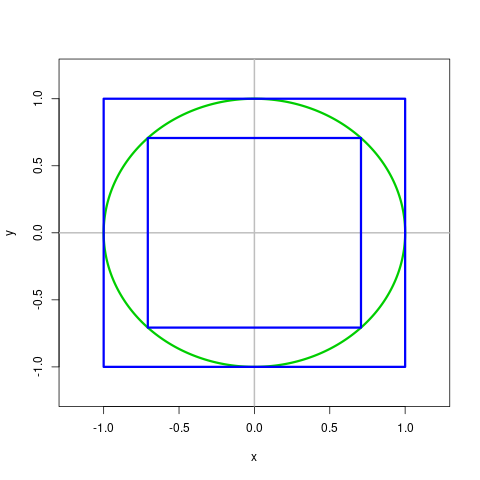
\includegraphics[width=.3\textwidth]{EquivalenceNorme-R2-2inf} & 
  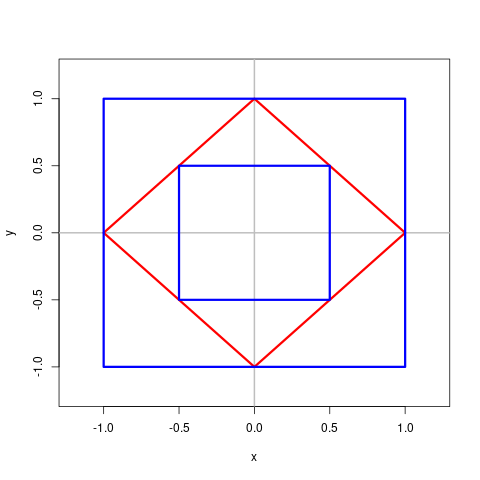
\includegraphics[width=.3\textwidth]{EquivalenceNorme-R2-1inf} & 
  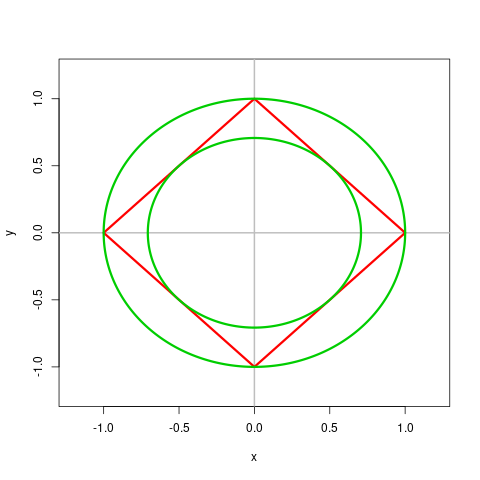
\includegraphics[width=.3\textwidth]{EquivalenceNorme-R2-12}
  \end{tabular}
  $$
%   $$
%   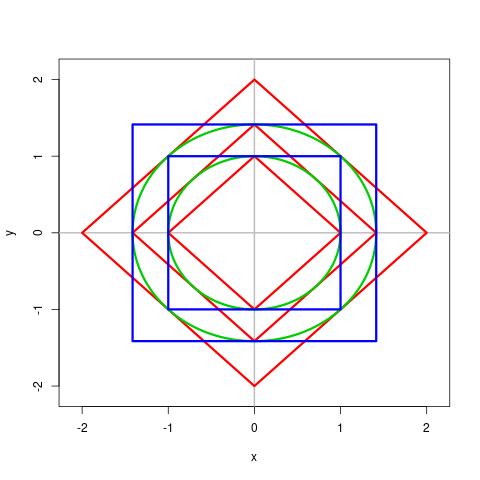
\includegraphics[width=.5\textwidth]{EquivalenceNorme-R2}
%   $$
}

